\documentclass[12pt,a4paper,openany]{book}
\usepackage[utf8]{inputenc}
\usepackage[spanish]{babel}
\usepackage{graphicx,lipsum,afterpage,caption}
\usepackage[left=3.0cm,right=3.0cm,top=3.0cm,bottom=3.0cm]{geometry}
\usepackage{mathptmx}
\usepackage{blindtext} 

\usepackage[Glenn]{fncychap} %Estilo para los capitulos, otros pueden ser: Sonny, Lenny, Glenn, Conny, Rejne, Bjarne, Bjornstrup

\usepackage{amssymb, amsmath, amsbsy, amsfonts}    % ECUACIONES Y SÍMBOLOS MATEMÁTICOS
\usepackage{listings} % PERMITE AGREGAR CÓDIGO DE LENGUAJES  DE PROGRAMACIÓN (DOCUMENTACIÓN EN GOOGLE)
\usepackage{emptypage}                   % QUITA LOS ENCABEZADOS Y PIES DE PÁGINA EN LAS HOJAS VACÍAS PRODUCIDAS POR LA IMPRESIÓN A DOS CARAS
\usepackage{wrapfig}                    % to include figure with text wrapping around it
% \usepackage[bf,SL,BF]{subfigure}         % Permite crear figuras múltiples
\usepackage{makeidx}                     % Contiene los macros para indexar en un glosario
\usepackage{mathdots}                    % para el comando \iddots
\usepackage{mathrsfs}                    % para formato de letra en ecuaciones
\raggedbottom                            %Evita que LaTeX distribuya los espacios en blanco sobre la página, en lugar de eso los envía al fondo
\usepackage{eucal}
\usepackage{float}
\usepackage{color}
\usepackage[perpage]{footmisc}
\usepackage{ifthen}
\usepackage{cite}
\usepackage{multicol} % for pages with multiple text columns, e.g. References
\setlength{\columnsep}{20pt} % space between columns; default 10pt quite narrow
\usepackage[nottoc]{tocbibind} % correct page numbers for bib in TOC, nottoc suppresses an entry for TOC itself
%\usepackage{nextpage}
% \usepackage{titlesec}
%\usepackage[siunitx]{circuitikz} %para circuitos
%\usepackage[makeroom]{cancel}%Para cancelar términos en modo matemático
%\usepackage{cleveref}           %COMO UNA FORMA DE REFERENCIAR TABLAS, ECUACIONES, ETC. -->http://mirror.utexas.edu/ctan/macros/latex/contrib/cleveref/cleveref.pdf
\pagenumbering{roman}

\usepackage{algpseudocode}
\usepackage{algorithm}
\usepackage{listings}
\usepackage{color}
\definecolor{gray97}{gray}{.97}
\definecolor{gray75}{gray}{.75}
\definecolor{gray45}{gray}{.45}

\usepackage{listings}
\lstset{ frame=Ltb,
framerule=0pt,
aboveskip=0.5cm,
framextopmargin=3pt,
framexbottommargin=3pt,
framexleftmargin=0.4cm,
framesep=0pt,
rulesep=.4pt,
backgroundcolor=\color{gray97},
rulesepcolor=\color{black},
%
stringstyle=\ttfamily,
showstringspaces = false,
basicstyle=\small\ttfamily,
commentstyle=\color{gray45},
keywordstyle=\bfseries,
%
numbers=left,
numbersep=15pt,
numberstyle=\tiny,
numberfirstline = false,
breaklines=true,
}

% minimizar fragmentado de listados
\lstnewenvironment{listing}[1][]
{\lstset{#1}\pagebreak[0]}{\pagebreak[0]}

\lstdefinestyle{consola}
{basicstyle=\scriptsize\bf\ttfamily,
backgroundcolor=\color{gray75},
}

\lstdefinestyle{C}
{language=C,
}


%%%%%%%%%%%%%%%%%%%%%%%%%%%%%%%%%%%%%%%%%%%%%%%%%%%%%%%%%%%%%%%%%%%%%%%%%%%%%%%%
%                                   DATOS                                      %
%%%%%%%%%%%%%%%%%%%%%%%%%%%%%%%%%%%%%%%%%%%%%%%%%%%%%%%%%%%%%%%%%%%%%%%%%%%%%%%%
\author{Marco Antonio Aguilar Gallardo}
\title{Tesis UNAQ}



\begin{document}
\frontmatter
%%%%%%%%%%%%%%%%%%%%%%%%%%%%%%%%%%%%%%%%%%%%%%%%%%%%%
%                   PORTADA                         %
%%%%%%%%%%%%%%%%%%%%%%%%%%%%%%%%%%%%%%%%%%%%%%%%%%%%%

\begin{titlepage}
	\begin{center}
		{\Huge Universidad Aeronáutica en Querétaro}
		\vspace{1cm}
		\begin{figure}[h]
			\centering
			\includegraphics[scale=0.6]{Portada/UNAQ_logo.png}			
		\end{figure}
	\end{center}

\end{titlepage}


%%%%%%%%%%%%%%%%%%%%%%%%%%%%%%%%%%%%%%%%%%%%%%%%%%%%%
%                  PRÓLOGO                          %
%%%%%%%%%%%%%%%%%%%%%%%%%%%%%%%%%%%%%%%%%%%%%%%%%%%%%
\include{Agradecimientos/Dedicatoria}
\include{Agradecimientos/Agradecimientos}

%%%%%%%%%%%%%%%%%%%%%%%%%%%%%%%%%%%%%%%%%%%%%%%%%%%%%
%                   ÍNDICES                         %
%%%%%%%%%%%%%%%%%%%%%%%%%%%%%%%%%%%%%%%%%%%%%%%%%%%%%
%Esta sección genera el índice
\pagestyle{headings}
\setcounter{tocdepth}{4}
\setcounter{secnumdepth}{5}
% \setcounter{secnumdepth}{3} % organisational level that receives a numbers
% \setcounter{tocdepth}{3}    % print table of contents for level 3
% \tableofcontents            % Genera el índice 
%: ----------------------- list of figures/tables ------------------------
\listoffigures              % Genera el ínidce de figuras, comentar línea si no se usa
\listoftables               % Genera índice de tablas, comentar línea si no se usa

%%%%%%%%%%%%%%%%%%%%%%%%%%%%%%%%%%%%%%%%%%%%%%%%%%%%%
%                   CONTENIDO                       %
%%%%%%%%%%%%%%%%%%%%%%%%%%%%%%%%%%%%%%%%%%%%%%%%%%%%%
\mainmatter
%\setcounter{equation}{0}
\chapter{Introducci\'on}
 	Este capítulo cubre los antecedentes de esta tesis, así como sus propósitos, objetivos y limitaciones originales
\section{Preámbulo}
El incremento reciente del uso de cámaras digitales en sistemas UAVs para el uso de producciones profesionales cinematográficas ha hecho que diversos científicos e ingenieros estén interesados en diseñar controladores para estabilizar la posición de referencia de dichas cámaras con el objetivo de mitigar la mayor cantidad de ruido en las filmaciones.\\
El desarrollo de algoritmos genéticos ha favorecido en la implementación de controladores para los sistemas estabilizadores por lo que ha dado apertura a múltiples creaciones de algoritmos con la finalidad de obtener el mejor controlador con respecto al tiempo de respuesta. \\
Debido a la versatilidad de los UAVs, la implementación de una cámara no solo se limita al uso cinematográfico, va más allá, un ejemplo es la investigación realizada por Georgia Tech UAV quienes dirigen su trabajo hacia la navegación mediante un control de visión artificial.  

\section{Objetivos}
\subsection{Objetivo general}
Diseñar, simular y programar un controlador de estabilidad para un sistema gimbal de dos grados de libertad mediante el uso de visión artificial para detectar figuras geométricas en un marco de referencia inercial.
\subsection{Objetivos espec\'ificos}
\begin{itemize}
\item Obtener el modelo matemático de un estabilizador gimbal de dos grados de libertad, con base en la propuesta realizada por Maher Abdo.
\item Diseñar un controlador autónomo con base en el modelo matemático previamente obtenido, para estabilizar la superficie del sistema gimbal y con ello mitigar las perturbaciones de entrada. 
\end{itemize}

\section{Planteamiento y justificaci\'on}
El trabajo presentado en esta tesis tiene su justificación académica, porque durante las fases del modelado matemático, diseño e implementación del controlador y aplicación de técnicas de visión artificial engloba de manera concreta los conocimientos adquiridos relacionados al campo de los sistemas embebidos, tales como, electrónica de control, control en tiempo continuo y discreto y además se integra a estudios aerodinámicos, debido a que la gimbal fue colocada en un sistema UAV.








\chapter{Marco Téorico}
En este capitulo desarrolla la teoría que fundamenta el proyecto de investigación con base
en el problema previamente descrito.\\
Antes de entrar a la teoría es necesario entender cuales son las fases del proyecto y
el porque de ellas.
La siguiente imagen muestra la similitud entre el sistema de adquisición de datos
de un humano y la de un sistema digital.
\begin{center}
    
\includegraphics[width=0.65\textwidth]{Capitulo2/Fig1.eps}       
    \captionof{figure}{Similitudes entre humano y computadora}\label{Fig1}
\end{center}
Donde se observa un diagrama de flujo que empieza con la adquisición de datos, en este
caso la captura de una imagen, posterior se hace un procesamiento, es decir, se le da
sentido a los datos, y finalmente se hace una acción con base en la tarea que el procesador
ha generado.

\section{Óptica}
La visión artificial surge de un amplio estudio probabilístico y matemático del 
procesamiento de imágenes digitales, pero sobre todo de análisis humanos y de la 
intuición ya que de estas últimas el ingeniero hace selección de entre una u otra 
técnica. Esta elección se basa usualmente en juicios visuales subjetivos.\\
Entender los conceptos básicos de la percepción humana es entonces pertinente, donde 
la Óptica nos ayudará a entender mejor como es que el ojo humano percibe y como lo 
hace una cámara. \\
La función de la óptica de una cámara es captar los rayos luminosos y concentrarlos 
sobre el sensor sensible de la cámara de vídeo. Después de determinar el tipo de 
iluminación que mejor se adecua al problema, la elección de una óptica u otra influirá 
en la calidad de la imagen y el tamaño de los objetos.
\subsection{Estructura del ojo humano}
\begin{itemize}
\item Cornea: La córnea es una estructura del ojo que permite el paso de la luz 
desde el exterior al interior del ojo y protege el iris y el cristalino. Posee 
propiedades ópticas de refracción y para garantizar su función debe ser transparente 
y es necesario que mantenga una curvatura adecuada.
\item Esclerótica: Es el recubrimiento exterior blanco del ojo. La esclerótica le da 
su color blanco al globo ocular.
\item Coroides: Es la capa de vasos sanguíneos y tejido conectivo entre la parte blanca del ojo y la retina (en la parte posterior del ojo). Es parte de la úvea y suministra los nutrientes a las partes internas del ojo.
\item Cuerpo ciliar: Es una estructura circular que es una prolongación del iris, la 
parte de color del ojo. También contiene el músculo ciliar, el cual cambia la forma 
del cristalino cuando los ojos se enfocan en un objeto cercano. Este proceso se 
denomina acomodación.
\item Diafragma Iris: que se expande o contrae para controlar la cantidad de luz que 
entra en el ojo. La apertura central del iris, llamada pupila, varía su diámetro de 2 
a 8mm. El frente del iris contiene el pigmento visible del ojo, y la parte trasera 
contiene un pigmento negro.
\item Cristalino: El cristalino es “la lente” del ojo y sirve para enfocar, ayudado 
por los músculos ciliares. El cristalino es una lente que actúa como una lente 
biconvexa, lenticular, flexible y avascular, cuya principal función es la de enfocar 
los objetos en las distintas distancias correctamente.
\item Retina: Es la capa de tejido sensible a la luz que se encuentra en la parte 
posterior globo ocular. Las imágenes que pasan a través del cristalino del ojo se 
enfocan en la retina. La retina convierte entonces estas imágenes en señales eléctricas
y las envía por el nervio óptico al cerebro.
\end{itemize}
\subsection{Formación de imágenes en el ojo}
En una cámara fotográfica se recibe la luz que traspasa el diafragma, pasa por los 
cristales de la cámara hasta llegar al CCD(Charge Coupled Device o, en español, 
Dispositivo de Carga Acoplada) o sensor, que es donde se forma la imagen correcta y se 
envía al procesador.\\
Algo similar pasa en el ojo, la pupila es el diagrama natural que filtra la luz que 
entra en el ojo, pasa por la lente (el cristalino)  que converge los rayos hasta 
llegar a la retina, que es la estructura que tiene las células fotosensibles y dónde 
se produce la imagen, y a través del nervio óptico se transporta la información al 
cuerpo geniculado, que es la parte del cerebro donde se produce la visión.\\
El ojo esta formado de dos componentes principales:
\begin{itemize}
\item Componentes ópticos: permiten la formación de la imagen en la retina y son los 
siguientes: la córnea, el cristalino, la pupila, el humor acuoso y el humor vítreo que 
permiten la formación de una imagen en la retina.
\item Componentes neurológicos: son los que transforman la información óptica en 
eléctrica y transmiten la información al cuerpo geniculado lateral. Estos componentes 
son la retina y el nervio óptico.
\end{itemize}

\section{Procesamiento de datos}
Este trabajo de investigación se basa en el procesamiento de datos usando un framework
llamado ROS (del inglés Robot Operating System).
\subsection{ROS}
Un sistema de comunicación es a menudo una de las primeras necesidades que surgen al 
implementar una nueva aplicación de robot. El sistema de mensajería integrado y 
probado de ROS ahorra tiempo al administrar los detalles de la comunicación entre 
los nodos distribuidos a través del mecanismo anónimo de publicación / suscripción. 
Otro beneficio de usar un sistema de paso de mensajes es que te obliga a implementar 
interfaces claras entre los nodos en tu sistema, mejorando así la encapsulación y 
promoviendo la reutilización de código. La estructura de estas interfaces de mensajes 
se define en el mensaje IDL (Lenguaje de descripción de interfaz).\\
Decidí usar ROS porque crear un software de robot verdaderamente robusto y de uso 
general es difícil. Desde la perspectiva del robot, los problemas que parecen triviales
para los humanos a menudo varían enormemente entre instancias de tareas y entornos. 
Hacer frente a estas variaciones es tan difícil que se necesita apoyo de un sistema
de comunicación.\\
ROS tiene tres niveles de conceptos: el nivel del sistema de archivos, el nivel del gráfico 
de cómputo y el nivel de la comunidad. ~\cite{ROS}
\subsubsection{Nivel de sistemas de archivos de ROS}
Los conceptos de nivel de sistema de archivos cubren principalmente los recursos de ROS que 
encuentra en el sistema, tales como:
\begin{itemize}
    \item \textbf{Paquetes}\\
    Los paquetes son la unidad principal para organizar el software 
    en ROS. Un paquete puede contener procesos (nodos) de tiempo de ejecución de ROS, 
    una biblioteca dependiente de ROS, conjuntos de datos, archivos de configuración o 
    cualquier otra cosa que se organice conjuntamente de manera útil. Los paquetes son 
    el elemento de construcción más atómico y el elemento de lanzamiento en ROS. Lo 
    que significa que lo más granular que puede construir y lanzar es un paquete.
\end{itemize}
\subsubsection{Nivel de gráfico de cómputo ROS}
En términos generales, ROS sigue la filosofía de desarrollo de software de Unix 
en varios aspectos clave. Esto tiende a hacer que ROS se sienta "natural" para los 
desarrolladores que vienen de un entorno Unix, pero algo "críptico" al principio 
para aquellos que han usado principalmente entornos de desarrollo gráfico en 
Windows o Mac OS X.~\cite{ROSMIKE}\\
Los sistemas ROS consisten en numerosos programas pequeños informáticos que se 
conectan entre sí e intercambian mensajes continuamente. Estos mensajes viajan 
directamente de un programa a otro.\\
Los conceptos básicos del gráfico de cómputo de ROS son nodos, mastaer, 
servidor de parámetros, mensajes, servicios, topics y bags, los cuales 
proporcionan datos al gráfico de diferentes maneras siguiendo la filosofia
antes descrita.
\begin{itemize}
    \item \textbf{Nodo}\\
    los nodos son procesos que realizan cálculos. ROS está diseñado para ser modular 
    a nivel de nodo; un sistema de control de robot generalmente comprende muchos nodos.
    \item \textbf{Master}\\
    Un programa intermedio que conecta nodos.
    \begin{center}
        \includegraphics[width=0.5\textwidth]{Capitulo2/Fig2.eps}       
        \captionof{figure}{Nodos conectados al Master}\label{Fig2}
    \end{center}
    
\end{itemize}
\chapter{Modelo Matematico}
En esta sección se analizara el modelo matemático que rige al sistema, pasando
por diferentes marcos de referencia, inercial, de la gimbal y de la camara.
\chapter{Vision Artificial}

\section{Camara}
Como se abordo al inicio de este proyecto, la cámara es la parte fundamental en
la captura de datos, suple la función de un ojo y depende de diversos
parámetros el que tengamos una captura de calidad. Para este trabajo profesional
la cámara que se utilizo fue la del fabricante HardKernel y que lleva de nombre
Ocam
\begin{center}
    \includegraphics[width=0.3\textwidth]{Capitulo4/Fig0_1.eps}       
    \captionof{figure}{Camara 'Ocam'}\label{Fig1}
\end{center}
Que tiene las siguientes especificaciones.
\begin{itemize}
    \item \textbf{Sensor:} CMOS image sensor.
    \item \textbf{Lente: } Lente estandar M12 distancia focal de 3.6mm.
    \item \textbf{Field of view: } 65 grados.
    \item \textbf{Tamaño del sensor: }0.25inch (3673.6 $\mu$m x 2738.4 $\mu$m)
    \item \textbf{Tamaño del pixel: } 1.4 $\mu$m x 1.4 $\mu$m.
    \item \textbf{Interfaz: }USB 3.0 Super-Speed.
    \item \textbf{Frame rate: }\\
    1920 x 1080 a 30fps, 1280 x 720 a45fps, 640 x 480 a30fps
\end{itemize}
El acceso directo a la memoria a través de USB 3.0 permite que los datos se 
escriban en la memoria principal sin pasar por la CPU. Reduce significativamente 
la carga de trabajo de la CPU.

\section{Algoritmo general}
\begin{algorithm}
    \caption{Algoritmo general del sistema de vision}
    \begin{algorithmic}[1]
        \State{Calibrar camara}
        \State{Capturar frame a 60fps}
        \State{Publicar frame en ROS}
        \State{Suscribirse al nodo publicador}
        \State{Convertir RGB a HSV}
        \State{Acotar el modelo HSV al color de elección}
        \State{Agregar filtro morfologico}
        \State{Obtener centroide de la figura obtenida en 6}
        \State{Publicar coordenadas del centroide}
    \end{algorithmic}
\end{algorithm}

% ---------------------------------------------------------------------------------------------------------
% *********************************************************************************************************
% *********************************************************************************************************
% ---------------------------------------------------------------------------------------------------------

\section{Calibración de camara}


% ---------------------------------------------------------------------------------------------------------
% *********************************************************************************************************
% *********************************************************************************************************
% ---------------------------------------------------------------------------------------------------------


\section{Comunicación con ROS}
En la sección de vision artificial se lanzan dos nodos, uno encargado de capturar y
publicar frames a 60hz y el otro que se suscribe a dicho nodo y realiza un procesamiento
con la información obtenida para posterior publicar coordenadas.
\begin{center}
    \includegraphics[width=0.6\textwidth]{Capitulo4/Fig0.eps}       
    \captionof{figure}{Nodos y topic}\label{Fig1}
\end{center}
En la figura 4.1 se puede observar dos nodos conectados por un topic llamado /Image
encargado de comunicar la imagen de un nodo a otro.
\subsection{Publisher}
Como vimos anteriormente opencv es una libreria open-source que se encarga del procesamiento
de imagenes, también abordamos un poco acerca de como ROS comunica nodos y los 
tipos de datos que puden ser publicados. Al hablar de que se va a publicar una imagen
estamos refiriendonos a una matriz que en este caso sera de 640 x 480.\\
ROS pasa las imágenes en su propio formato sensor\_msgs/Image , pero
en este caso usaremos ROS junto con las librerias de  OpenCV. CvBridge es una 
biblioteca ROS que proporciona una interfaz entre ROS y OpenCV.
\begin{center}
    
\includegraphics[width=0.5\textwidth]{Capitulo4/Fig1.eps}       
    \captionof{figure}{Comunicación entre opencv y ROS}\label{Fig1}
\end{center}
Al convertir un mensaje sensor\_msgs/Image en una imagen Cv, CvBridge 
reconoce dos casos de uso distintos:
\begin{itemize}
    \item Queremos modificar los datos en el lugar.\\
    \textbf{Tenemos que hacer una copia de los datos del mensaje ROS.}
    \item No modificaremos los datos.\\
    \textbf{Podemos compartir con seguridad los datos que posee el mensaje ROS en lugar de copiarlos.}
\end{itemize}
 
La entrada es el puntero del mensaje de imagen, así como un argumento de 
codificación opcional. La codificación se refiere al destino CvImage.\\
Para codificaciones de imágenes populares, CvBridge opcionalmente realizará 
conversiones de color o profundidad de píxeles según sea necesario. Para este proyecto
se utiliza bgr8: CV\_8UC3, es decir, que el orden del color es Azul, Verde y Rojo.\\
Con el fin de entender este nodo se hizo el siguiente diagrama de flujo:
\begin{center}
    \includegraphics[width=0.35\textwidth]{Capitulo4/publisher.eps}       
    \captionof{figure}{Diagrama de flujo del programa publisher}\label{Fig5}
\end{center}
El codigo se encuentra en la parte del Apendice A, 'codigo1'

\subsection{Subscriber}
Este nodo tiene dos funciones principales, Suscribirse al nodo publisher y publicar
un array de tamaño 2 tipo entero que guardara las coordenadas en X y Y del centroide
del target.\\
El proceso que se ejecuta se vera más a detalle en las siguientes secciones de este
capitulo.

% ---------------------------------------------------------------------------------------------------------
% *********************************************************************************************************
% *********************************************************************************************************
% ---------------------------------------------------------------------------------------------------------

\section{Espacio de color}
Como se puede apreciar en el algoritmo general, el paso 5 es el cambio de espacio de color
de RGB a HSV, además ya sabemos el porque es mejor generar colores partiendo del
modelo HSV. Así que lo que ahora sigue es la implementación en código y las pruebas
que se hicieron para tener un rango de colores y así tener una base de datos a la
cual recurriremos después.\\
Debido a que no hay un solo color azul o rojo, etc, si no más bien un rango que cubre
la gama de azules, amarillo, naranja, etc. Por esa razón se hicieron pruebas para
determinar los valores HSV que corresponden a los siguientes colores: Amarillo, Azul,
Rojo, Verde y Naranja y de esta manera a la hora de seguir un objetivo de dado color
el sistema no tenga problemas en reconocer esa gama de color.
\subsection{Prueba de amarillo}
\begin{center}
    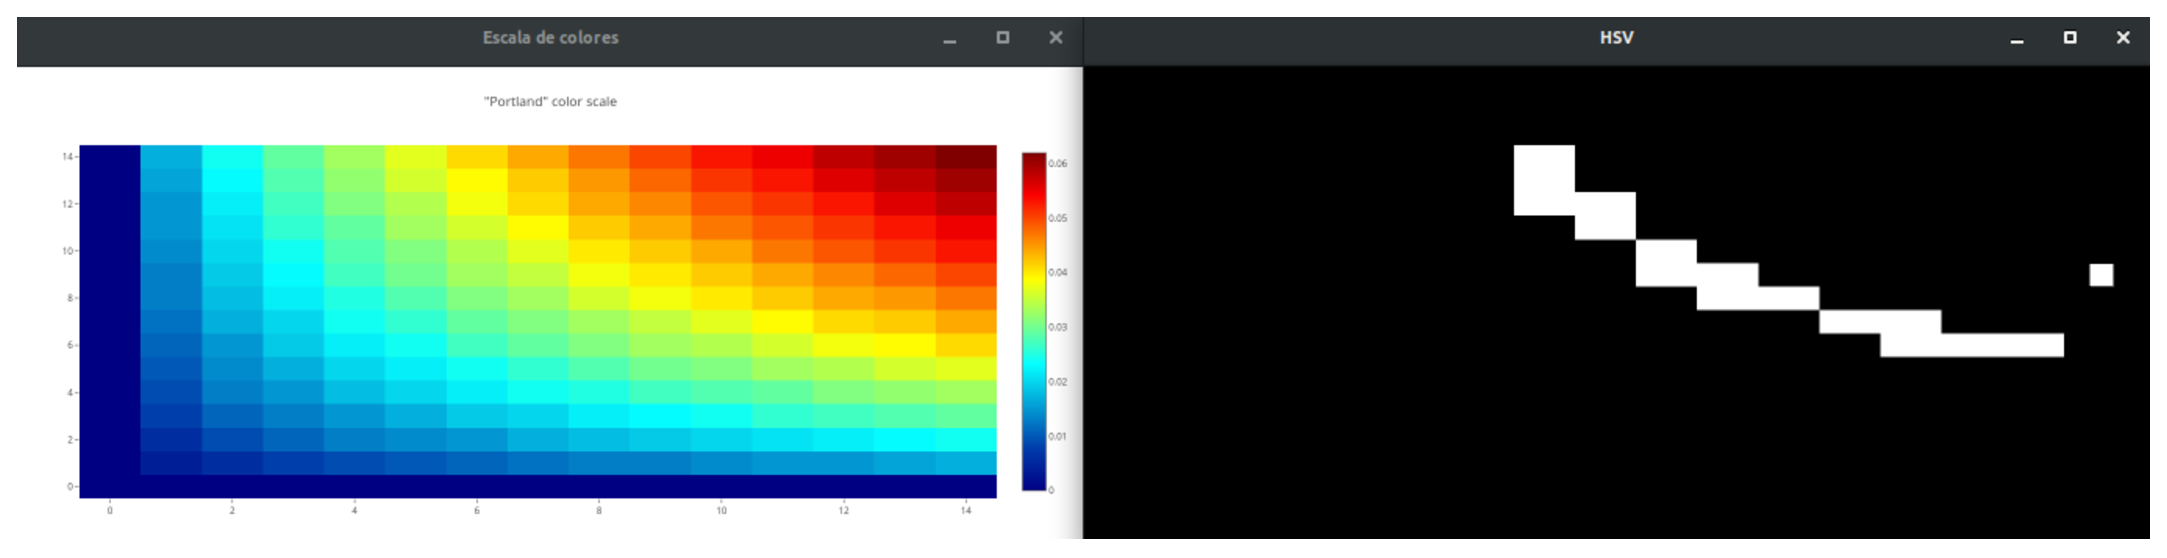
\includegraphics[width=1.0\textwidth]{Capitulo4/HSV_amarillo.eps}       
    \captionof{figure}{Pruebas para color amarillo}\label{Fig6}
\end{center}
Los valores para el rango que considere amarillo son:\\
H minimo  = 25\\
S minimo = 50 \\
V minimo = 50 \\
H maximo = 32 \\
S maximo = 255 \\
V maximo = 255 

\subsection{Pruebas de color Rojo}
El color rojo, en OpenCV, tiene los valores de tono aproximadamente en 
el rango de 0 a 10 y 160 a 180.\\
prueba


%%%%%%%%%%%%%%%%%%%%%%%%%%%%%%%%%%%%%%%%%%%%%%%%%%%%%
%                   REFERENCIAS y Apendices                 %
%%%%%%%%%%%%%%%%%%%%%%%%%%%%%%%%%%%%%%%%%%%%%%%%%%%%%
\backmatter
% existen varios estilos de bilbiografía, pueden cambiarlos a placer
% \printbibliography
% \bibliographystyle{apalike} % otros estilos pueden ser abbrv, acm, alpha, apalike, ieeetr, plain, siam, unsrt
\include{ApendiceA/ApendiceA}
\bibliography{Bibliografia/Referencias}{}              %Archivo .bib
\bibliographystyle{apalike}
\end{document}